%%%%%%%%%%%%%%%%%%%%%%%%%%%%%%%%%%%%%%%%%
% Arsclassica Article
% LaTeX Template
% Version 1.1 (10/6/14)
%
% This template has been downloaded from:
% http://www.LaTeXTemplates.com
%
% Original author:
% Lorenzo Pantieri (http://www.lorenzopantieri.net) with extensive modifications by:
% Vel (vel@latextemplates.com)
%
% License:
% CC BY-NC-SA 3.0 (http://creativecommons.org/licenses/by-nc-sa/3.0/)
%
%%%%%%%%%%%%%%%%%%%%%%%%%%%%%%%%%%%%%%%%%

%----------------------------------------------------------------------------------------
%	PACKAGES AND OTHER DOCUMENT CONFIGURATIONS
%----------------------------------------------------------------------------------------

\documentclass[
10pt, % Main document font size
letterpaper, % Paper type, use 'letterpaper' for US Letter paper
oneside, % One page layout (no page indentation)
%twoside, % Two page layout (page indentation for binding and different headers)
headinclude,footinclude, % Extra spacing for the header and footer
english
]{article}

%%%%%%%%%%%%%%%%%%%%%%%%%%%%%%%%%%%%%%%%%
% Arsclassica Article
% Structure Specification File
%
% This file has been downloaded from:
% http://www.LaTeXTemplates.com
%
% Original author:
% Lorenzo Pantieri (http://www.lorenzopantieri.net) with extensive modifications by:
% Vel (vel@latextemplates.com)
%
% License:
% CC BY-NC-SA 3.0 (http://creativecommons.org/licenses/by-nc-sa/3.0/)
%
%%%%%%%%%%%%%%%%%%%%%%%%%%%%%%%%%%%%%%%%%

%----------------------------------------------------------------------------------------
%	REQUIRED PACKAGES
%----------------------------------------------------------------------------------------

\usepackage[
nochapters, % Turn off chapters since this is an article        
beramono, % Use the Bera Mono font for monospaced text (\texttt)
eulermath,% Use the Euler font for mathematics
pdfspacing, % Makes use of pdftex’ letter spacing capabilities via the microtype package
dottedtoc % Dotted lines leading to the page numbers in the table of contents
]{classicthesis} % The layout is based on the Classic Thesis style

\usepackage{arsclassica} % Modifies the Classic Thesis package

\usepackage[T1]{fontenc} % Use 8-bit encoding that has 256 glyphs

\usepackage[utf8]{inputenc} % Required for including letters with accents

\usepackage{graphicx} % Required for including images
\graphicspath{{Figures/}} % Set the default folder for images

\usepackage{enumitem} % Required for manipulating the whitespace between and within lists

\usepackage{lipsum} % Used for inserting dummy 'Lorem ipsum' text into the template

\usepackage{subfig} % Required for creating figures with multiple parts (subfigures)

\usepackage{amsmath,amssymb,amsthm} % For including math equations, theorems, symbols, etc

\usepackage{varioref} % More descriptive referencing

%----------------------------------------------------------------------------------------
%	THEOREM STYLES
%---------------------------------------------------------------------------------------

\theoremstyle{definition} % Define theorem styles here based on the definition style (used for definitions and examples)
\newtheorem{definition}{Definition}

\theoremstyle{plain} % Define theorem styles here based on the plain style (used for theorems, lemmas, propositions)
\newtheorem{theorem}{Theorem}

\theoremstyle{remark} % Define theorem styles here based on the remark style (used for remarks and notes)

%----------------------------------------------------------------------------------------
%	HYPERLINKS
%---------------------------------------------------------------------------------------

\hypersetup{
%draft, % Uncomment to remove all links (useful for printing in black and white)
colorlinks=true, breaklinks=true, bookmarks=true,bookmarksnumbered,
urlcolor=webbrown, linkcolor=RoyalBlue, citecolor=webgreen, % Link colors
pdftitle={}, % PDF title
pdfauthor={\textcopyright}, % PDF Author
pdfsubject={}, % PDF Subject
pdfkeywords={}, % PDF Keywords
pdfcreator={pdfLaTeX}, % PDF Creator
pdfproducer={LaTeX with hyperref and ClassicThesis} % PDF producer
} % Include the structure.tex file which specified the document structure and layout
\usepackage[letterpaper]{geometry}
\geometry{verbose,tmargin=1in,bmargin=1.3in,lmargin=1.45in,rmargin=1.45in}

\hyphenation{Fortran hy-phen-ation} % Specify custom hyphenation points in words with dashes where you would like hyphenation to occur, or alternatively, don't put any dashes in a word to stop hyphenation altogether

%----------------------------------------------------------------------------------------
%	TITLE AND AUTHOR(S)
%----------------------------------------------------------------------------------------

\title{\normalfont\spacedallcaps{CIS 559 Project 3:\break Gunslinger}} % The article title

\author{\spacedlowsmallcaps{Ian Sibner, David Liao, Nikhil Roy}} % The article author(s) - author affiliations need to be specified in the AUTHOR AFFILIATIONS block

\date{20 October 2015} % An optional date to appear under the author(s)

%----------------------------------------------------------------------------------------
\setlength\parindent{0pt}
\setlength{\parskip}{1em}

\usepackage[section]{placeins}

\begin{document}

%----------------------------------------------------------------------------------------
%	HEADERS
%----------------------------------------------------------------------------------------

\renewcommand{\sectionmark}[1]{\markright{\spacedlowsmallcaps{#1}}} % The header for all pages (oneside) or for even pages (twoside)
%\renewcommand{\subsectionmark}[1]{\markright{\thesubsection~#1}} % Uncomment when using the twoside option - this modifies the header on odd pages
\lehead{\mbox{\llap{\small\thepage\kern1em\color{halfgray} \vline}\color{halfgray}\hspace{0.5em}\rightmark\hfil}} % The header style

\pagestyle{scrheadings} % Enable the headers specified in this block

%----------------------------------------------------------------------------------------
%	TABLE OF CONTENTS & LISTS OF FIGURES AND TABLES
%----------------------------------------------------------------------------------------

\maketitle % Print the title/author/date block

\setcounter{tocdepth}{2} % Set the depth of the table of contents to show sections and subsections only

\tableofcontents % Print the table of contents

\listoffigures % Print the list of figures

% \listoftables % Print the list of tables

%----------------------------------------------------------------------------------------
%	ABSTRACT
%----------------------------------------------------------------------------------------

\section{Introduction} % This section will not appear in the table of contents due to the star (\section*)

Gunslinger is an $n$-player game where each player is initialize with two disjoint sets of $f$ friendly players (\textit{friends}) and $e$ enemy players (\textit{enemies}). This implies that $e + f < n$ since the player will not have itself as a friend or enemy. The friend relationship is symmetric, so if A is a friend of B, then B is a friend of A; the enemy relationship, however, may be asymmetric.

Each turn, each player can fire one shot in an attempt to kill another player. However, a player is not killed unless two players shoot it simultaneously. Once dead, a player can no longer shoot. The game ends when the set of living players remains unchanged for 10 rounds in a row, whether or not players are still shooting. Each players' objective is have the highest number of points at the end of the round. Points are awarded as follows:
\begin{enumerate}
  \item One point for surviving until the end of the round.
  \item One point for each surviving friend (maximum $f$).
  \item One point for each dead enemy (maximum $e$).
\end{enumerate}

Players retain perfect information about who shot whom in previous rounds.

\section{Initial Insights and Observations}

Immediately, our team observed several key features about the game.

\begin{enumerate}
  \item The information available to organisms would be very limited. They can only `see' in four directions, and could only detect food (or lack of food) and other organisms' states. So strategies that required non-local knowledge or multi-organism coordination would be difficult to implement.
  \item Staying put is much cheaper than moving since $v \geq 1$. Also, for the majority of the setups we considered, we had $v \geq 20$. Therefore, an organism should stay put more often than it moves.
  \item For all setups, we had $q \geq p$. This means that food tended to `collect' in certain squares, rather than being widely distributed on empty squares.
  \item A player with fewer individual organisms tends to die out faster, due to the random nature of food spawning. So it pays to try and reproduce fairly often.
  \item Reproducing produces two organisms with half the energy of the original, so the more energy an organism has when it reproduces, the more likely both offspring will survive.
\end{enumerate}

These insights guided our strategy throughout and allowed us to focus on the most important aspects of the game.

\section{Strategies and Concepts}

\subsection{XOrganism}

XOrganism was our first attempt, so we tried to create an organism that would survive on its own in a variety of conditions. The goal was to have a good survival rate in ``desert'' conditions, where $p \leq 0.005$. We did this in several ways.

First, we defined the idea of an organism being `sated'. In effect, a sated organism is close enough to its maximum energy that it is not in immediate need of food. There are many possible definitions for satiety; we initially defined an organism as sated if $Energy_{organism} \geq M - u$. This was a fairly intuitive definition: an organism is sated if eating one more unit of food would fill it up completely.

For movement, we tried to stay put very often because it only cost 1 unit of energy. We only moved under a few conditions:
\begin{enumerate}
  \item An adjacent square has food, and the organism is not `sated'. The rationale behind this movement pattern is fairly obvious - organisms tend to survive longer if they seek out food.
  \item The organism is `sated', but its square still has food. The idea here was to be \textit{courteous}, and allow other organisms who might need that food to jump on it.
  \item The organism has not found food in 20 turns. In this case, it moves in a random direction to try to look for food it might have missed.
\end{enumerate}
For reproduction, our organism was similarly simple. If the player is sated, then there is a 70\% chance of reproducing in a random direction. This ensures that when an organism does reproduce, both offspring have about half of their maximum energy, giving them a better chance of survival.

This organism tended to do pretty well on its own, surviving in about 30\% of our test runs with $p=0.005$. However, it performed significantly worse than other players in configurations where food was readily available. Worse, it tended to get ``choked out'' by more aggressive players, who would often take advantage of its courteous moves to take the food for themselves and reproduce. So, while it was a fairly good start, we needed to make some changes before XOrganism could be competitive.

\subsection{Protective Farmer}
The Protective Farmer was a reaction to the results of the preliminary test run during the first several classes. XOrganism was not faring so well later on in games with other, more aggressive, players, even when it did well in the early stages of the game. As well, due to XOrganism's courteous moves, it would lose valuable coverage of the food-populated cells on the board.

The Protective Farmer was an experiment to see if these issues could be mitigated by a completely different strategy. The core idea behind the Farmer was that if there were four organisms on each adjacent cell to a cell with food, they could all `farm' this cell. Staying off of the cell would allow it to duplicate freely, while the adjacency pattern would prevent opposing players from reaching the food source.

The initial stage of the Protective Farmer, before farming a food source, is to find a source of food that could support this configuration. In games with more organisms, many of the cells were covered up quickly, or enemy organisms prevented the Farmer from reaching other cells. The solution for this problem in Protective Farmer was almost the exact opposite of the movement strategy in XOrganism. The Farmer would move onto a new, unexplored cell on every turn (unless it needed food). It's goal was to find a cell with greater than four units of food on it as the Farmer may have needed to eat and will have to reproduce three times all without eating up the remainder of the food.

Once it found a satisfactory source food cell it transitioned into a building phase. The Farmer would look at all adjacent tiles and see if any were filled. If more than two were empty, then the farmer reproduces a wall onto one of those cells. This continues until there is only one cell left uncovered, which the Farmer simply moves to (instead of reproducing on to) to become the final wall. This Farmer organism and the newly spawned Farmer players are set to a Protective mode. This means that the organisms will stay still on their own cell unless they need food. If they do, they will attempt to move inwards. Once they replenish their energy, they move back onto the open cell they left earlier. In addition, when they move into the center cell, they also transition back to the building phase to fill any gaps in the wall that may have formed if any other Farmer organisms died off.

\subsection{David's Revenge's Revenge}

As the name suggests, David's Revenge's Revenge (DRR for short) was built directly on top of David's Revenge. Determining who to shoot is the exact same as David's Revenge: when DRR shoots, it will shoot the enemy who shot it most in previous rounds. However, unlike David's Revenge, DRR does not shoot whenever it can. It uses a logistic function in order to determine a \textit{shooting percentage}, and then shoots with a probability equal to this function value.

The intuition behind the logistic function is that in situations with lots of friends, it is better to be conservative with shooting. The friends of the enemy you shot are likely to retaliate in subsequent rounds, so a player that is too aggressive in these situations is likely to die. However, in situations with few friends, being aggressive makes more sense because retaliation is unlikely. This applies regardless of the number of actual enemies; it generally pays off to target neutral players as well, as long as there are few friends, because it improves a players' \textit{relative} ranking compared to other players. It was noted by Spriha that this might bring down a players' ranking in certain situations because it would eliminate another player's enemy; however, as we will see in the results section, we actually did quite well in situations where there were many enemies.

Thus we used the ratio of non-friends to players as the independent variable in the logistic function: $x = \dfrac{n - f}{n}$. Then the shooting percentage is calculated as $P = \dfrac{1}{1 + e^{-\frac{x - \mu}{\beta}}}$, where $\beta$ and $\mu$ govern the steepness and the mean of the distribution respectively. Initially, our logistic curve had $\beta=0.07,\mu=0.07$ (see Figure 1). However, we wanted to find the best-performing combination, so we systematically tried different combinations of $\mu$ and $\beta$ to find out which produced the best rank. In the end, we found that $\beta=0.06,\mu=0.4$ (see figure 2) was the best performing. This curve was more aggressive than the original curve; it appears that shooting more often improves performance even at relatively low non-friend to players ratio, reaching 90\% at an x-value of just 60\%.

\begin{figure}[h]
\centering
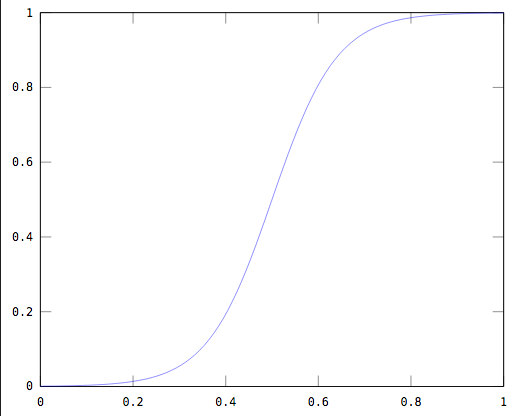
\includegraphics[width=0.8\columnwidth]{old-logistic-curve.png}
\caption[Initial logistic curve with $\beta=0.07,\mu=0.5$]{Initial Logistic Curve with $\beta=0.07,\mu=0.5$}
\label{fig:gallery2}
\end{figure}

\begin{figure}[h]
\centering
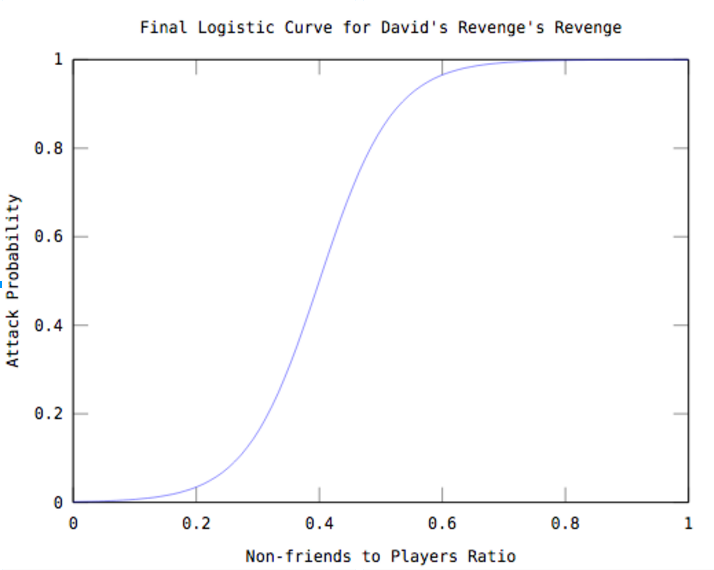
\includegraphics[width=0.8\columnwidth]{new-logistic-curve.png}
\caption[Final logistic curve with $\beta=0.06,\mu=0.4$]{Final logistic curve with $\beta=0.06,\mu=0.4$}
\label{fig:gallery3}
\end{figure}
\section{Implementation}

\subsection{XOrganism}

The implementation of XOrganism was fairly straightforward, as it only considered its current energy level and known parameter values. The only bit of state that was carried over (in addition to game state, such as current energy level) was the number of turns it had been alive (which was used in order to move every 20th turn to seek out more food). We first defined an \texttt{isSated} function (which just determined whether $Energy_{organism} \geq M - u$). Then, every turn, we did the following:

\begin{enumerate}
  \item If the organism was sated, we would reproduce with a probability of 70\%.
  \item If the organism did not reproduce, but still had food on its square and was sated, then it would move into an empty adjacent square - a courteous move designed to help other XOrganisms who might need food.
  \item If there was no food in its square, and the organism was not sated, then it would attempt to move into an adjacent square with food. Usually, if there was no food available, the organism would stay put. But every 20th turn (determined by the age counter), it would make a random move in order to seek out pockets of food that might be just beyond its field of vision.
\end{enumerate}

This implementation was very simple - only 100 lines of Java code. This is notable because this organism did tend to survive on its own, showing that even very simple heuristics can lead to acceptable results.

\subsection{Protective Farmer}
The implementation of Protective Farmer was divided up into several different phases. The Farmer uses external state to keep track of which phase of its lifecycle it's in, but this information is only used between players during the building phase.

The first phase was classified as the SEARCHING phase. Only the first organism would start out with this state. If the cell that the Farmer was on had no units of food, it would attempt to move in an unvisited direction with food. If there was no unvisited direction with food, then it would be an unvisited direction. If there was no remaining unvisited direction, then the Farmer would attempt to move in any open direction. These choices were calculated by filtering down the set of possible choices (from open directions to unvisited directions to unvisited directions with food) and then randomly picking a remaining option. The Farmer's visited steps were calculated by keeping track of its position relative to its point of birth. Once the Farmer takes a step, its previous position is added to a set of Points (later used in determining if the Farmer is attempting to visit a cell that has already been visited). One potential drawback to this strategy is that the Farmer won't be able to figure out the global coordinates of its position and therefore could be revisiting certain cells if it wraps around an edge during its life. As well, due to the random nature of direction selection, it is possible that the Farmer could trap itself inside its own path. In this case, the Farmer will look at only open directions as it will eventually have no other options. The Farmer will only stop if is hungry and needs food, or it find an adequate food source to start farming.

Once the Farmer finds a satisfactory (food units are greater than four) food source, it transitions into the CENTER phase. In this phase, the farmer looks at the adjacent tiles and looks to see if they are filled with other Farmers in the WALL phase. For this implementation, the WALL external state is an integer from three to six, so it is possible a malicious imposter could break this strategy. If more than two of these directions are empty, the Farmer reproduces in that direction, passing along this direction information to the new Farmer organism. There are four WALL states: WEST\_WALL(3), EAST\_WALL(4), NORTH\_WALL(5), and SOUTH\_WALL(6). If there is exactly one direction that is not protected by a wall, then the Farmer moves in that direction, becoming that wall.

All of the walls have the same logic for their phase. If they reach a minimum energy threshold they will attempt to move back onto the food source (transitioning into the CENTER phase as well). Otherwise, they will remain motionless. The minimum threshold is the movement cost $v$ plus nine times the stay cost (1). The absolute minimum survivable energy level is one more than the movement cost, because even if the organism can move to get food, it will not survive the move. The only other action a Farmer in the wall phase can take is reproduce (with some probability, just like XOrganism) away from the food source if the cell it is originally spawned on has food.

\subsection{SimplePlayer}
The implementation of Simple Player was true to its name, simple. It relied on the basic input parameters to the game and simple strategic calculations. Most of the behavior was identical to the XORganism, with only a few changes and improvements (which are listed below).

\begin{itemize}
  \item \textbf{Reproduction:} The more aggressive reproduction strategy was implemented from two angles.
    \begin{itemize}
      \item We increased the reproductive probability to 90\% after many trials of different values with other organisms in various configurations. Any higher, and the organism tended to overextend and die off; lower, and the organism would not spread fast enough to be competitive even on large boards.
      \item Simultaneously, we decreased the energy required to reproduce to $Energy_{organism} \geq M - 1.5 u$ - i.e., we changed the definition of ``sated'' to require slightly less energy. This tended to make  the organism much less conservative about reproduction, while still ensuring offspring had sufficient energy. The value of 1.5 was also determined to be an effective value through many trialss.
    \end{itemize}
    Therefore, on a given turn in the energy is greater than the new energy threshold, there is a 90\% chance of reproduction.
  \item \textbf{Movement:} The organisms performs the following checks for movement on a given turn.
  \begin{enumerate}
    \item If there is food on the square of the organism, then the organism stays put and eats.
    \item   If there is food on at least one of the squares, then it will move to a random surrounding square containing food.
    \item  If there is not food on any of the surrounding squares, then the organism, provided it has enough energy, will move to a random square. If the north square is available, then the organism will take it with probability 75\%.
  \end{enumerate}
\end{itemize}

\section{Results}
This project has many more configuration variables compared to the previous project (eight rather than two). However, the players were not generally aware of most of these changing parameters. As such, players were designed to function reasonably well in all cases, especially those where hidden parameters were set to extremes. The results from the several tournament runs are essentially a sampling of different viable configurations for this game. As well, there are two completely different tournament scenarios to consider. For these results, only the scenarios where the players were by themselves or in a group of the best six will be considered.

These tables include t-scores for SimplePlayer compared to all of the players involved. Significance, as used below, refers to significance with a confidence level of 95\% (against a t-score of 2.571).

\begin{figure}[h]
\centering
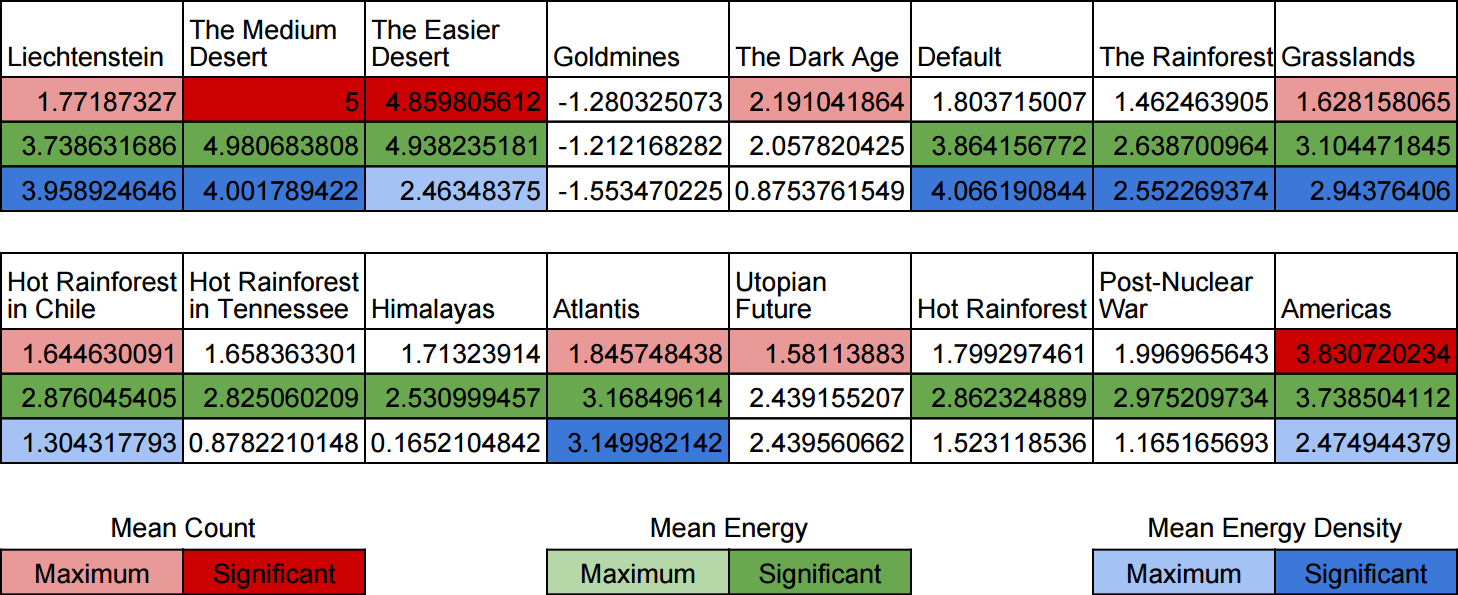
\includegraphics[width=0.8\columnwidth]{single-runs_table}
\caption[Table of t-score statistics for Single Run Tournaments]{t-score significance of count, energy, and energy density}
\label{fig:gallery2}
\end{figure}

We firstly consider the results from the single player tournaments (Figure 1), where each tournament was run with ony one player. From the results, it appears that SimplePlayer did exceptionally well when considering the total energy held on the board. SimplePlayer had a significantly greater amount of energy than any of the other five players in thirteen out of sixteen configurations. For many of these configurations, SimplePlayer also has a significantly greater or greatest energy density (Energy / Count). These successes are most likely due to a movement strategy that favors staying on, moving to, and reproducing to cells with food.

The one configuration from the single player tournaments that produced a remarkably poor performance from the SimplePlayer is Goldmines. This is due to the abnormally low value of $p$, which makes it very unlikely that a player standing still will ever see food before starving to death. Since it was more common that the SimplePlayer never had food spawn next to it, it most likely went extinct. Normally, the SimplePlayer is naturally optimized for low-$p$ conditions (seeking out food as a movement priority), but Goldmines is just too sparse of a configuration. If $p$ was slightly higher, SimplePlayer may have performed as well as it did in both The Medium Desert and The Easier Desert. Once SimplePlayer successfully managed the starting phase of a low-$p$ configuration, it ended up doing the best out of all six players included.

\pagebreak

\begin{figure}[h]
\centering
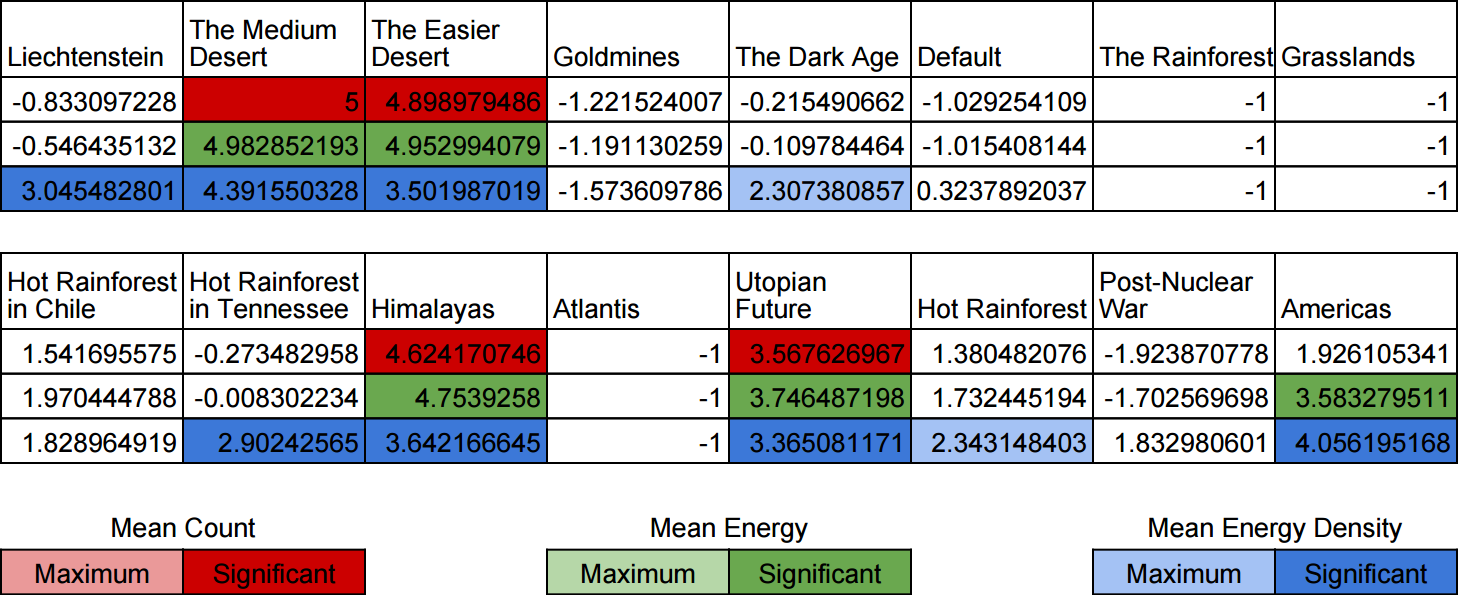
\includegraphics[width=0.8\columnwidth]{best6-runs_table}
\caption[Table of t-score statistics for Best Six Tournaments]{t-score significance of count, energy, and energy density}
\label{fig:gallery2}
\end{figure}

The results from the best six player tournaments (Figure 2) are very different from the single player tournaments. SimplePlayer only did well in several configurations: The Medium Desert, The Easier Desert, Himalayas, Utopian Future, and Americas. The reasoning for the successful performance of SimplePlayer has already been explained above. However, the remaining two configurations are very strange. SimplePlayer performed moderately well on Hot Rainforest, but for Utopian Future it was significantly greater than any other player. The main differences are an increase in $K$ and $u$ and a decrease in $v$. The addition of such mobility, combined with the incredible reward for finding food allowed SimplePlayer to function the best. Himalayas is a larger than default board, with a higher moving cost $v$. One reason that SimplePlayer performed so well is that the movement logic is set to only move when food is available, it is not wasteful with movement. This strategy allowed SimplePlayer to perform significantly greater than every other player on both The Medium Desert and The Easier Desert, as well as the Himalayas.

For the best six player configurations, there were noticeable declines in performance from the single player runs. Many of the configurations ended up being monopolized by one player (normally Group 4's FarmingPlayer), leaving very poor results for the SimplePlayer. However, despite the fact that many organism totals and organism energy levels were lower than the average produced by other organisms, the energy density was still fairly high (significant in some cases like Liechtenstein).



\section{Contributions}

We had two main contributions to the class strategy and discussion:
\begin{enumerate}
  \item \textbf{Importance of initial expansion -} We were one of the initial teams to implement a strategy, XOrganism, that demonstrated the lasting benefits of rapid initial yet sustainable reproduction. While were not the only team to arrive at this conclusion, it proved very important to many teams' strategies throughout the class.
  \item \textbf{Northward tendency -} Our team was the first team to recognize the downward trend in organism movement and implement a strategy to alter our movement with a directional tendency to increase longevity of organism survival.
\end{enumerate}

\section{Future Directions and Limitations}

\subsection{Faster Initial Spread}

Our players tended to do best on larger boards because of its high energy density. It tended not to overextend, unlike some other organisms which would tend to start dying frequently due to very aggressive population growth. But on small maps, this aggressive overextension was actually beneficial to these organisms, because they could ``choke out'' less aggressive competitors and dominate all food resources. Once their opponents went extinct, their organisms would settle into a steady state of lower population and energy compared to their initial population explosion. However, by that time, it was too late for slower-growing competitors like SimplePlayer.

Although an organism might not know the size of the board it starts on, we believe that our SimplePlayer could benefit from employing a more aggressive strategy \textit{only during the first part of the game}. The ideal length of this ``aggressive period'' might vary based on known map conditions, but based on our observations of population explosions in configurations where the total grid size was less than 1000, we believe that around 100 turns of aggressive expansion is usually sufficient to gain dominance over a large portion of the map. Once this period is up, we would switch to our current, more conservative strategy to take advantage of its natural tendency towards higher energy density. This would make our SimplePlayer much harder to choke out at the beginning, but would still allow it to take advantage of its effective conservative strategy after the intial territory grab. Following the initial population explosion, organisms that maintained aggression would tend to move more and use more energy, which would allow our less aggressive organisms to slowly chip away at their territory while maintaining a high average energy level.

\section{Acknowledgments}

The evolution of our players was heavily based on class discussion and iteration of our original ideas based on in-class runs. Group 2 was particularly helpful, due to its ``Rabbits'' strategy (later renamed to ``Harvey''). Their fast expansion - and the way they efficiently choked out our XOrganism and our first draft of SinglePlayer - convinced us of the need to be less cautious about our reproduction chances if we wanted to compete in high-food environments.

\section{Conclusion}

Overall we were happy with the progression of this project, particularly our SimplePlayer's performance on large boards or boards with high movement costs. We ended up with the highest population and overall energy in several of the tournament configurations, showing that good results could be achieved even with comparatively simple heuristics.
\end{document}
